%---------- Inleiding ---------------------------------------------------------

\section{Introductie}%
\label{sec:introductie}

% Waarover zal je bachelorproef gaan? Introduceer het thema en zorg dat volgende zaken zeker duidelijk aanwezig zijn:

% \begin{itemize}
%   \item kaderen thema
%   \item de doelgroep
%   \item de probleemstelling en (centrale) onderzoeksvraag
%   \item de onderzoeksdoelstelling
% \end{itemize}

% Denk er aan: een typische bachelorproef is \textit{toegepast onderzoek}, wat betekent dat je start vanuit een concrete probleemsituatie in bedrijfscontext, een \textbf{casus}. Het is belangrijk om je onderwerp goed af te bakenen: je gaat voor die \textit{ene specifieke probleemsituatie} op zoek naar een goede oplossing, op basis van de huidige kennis in het vakgebied.

% De doelgroep moet ook concreet en duidelijk zijn, dus geen algemene of vaag gedefinieerde groepen zoals \emph{bedrijven}, \emph{developers}, \emph{Vlamingen}, enz. Je richt je in elk geval op it-professionals, een bachelorproef is geen populariserende tekst. Eén specifiek bedrijf (die te maken hebben met een concrete probleemsituatie) is dus beter dan \emph{bedrijven} in het algemeen.

% Formuleer duidelijk de onderzoeksvraag! De begeleiders lezen nog steeds te veel voorstellen waarin we geen onderzoeksvraag terugvinden.

% Schrijf ook iets over de doelstelling. Wat zie je als het concrete eindresultaat van je onderzoek, naast de uitgeschreven scriptie? Is het een proof-of-concept, een rapport met aanbevelingen, \ldots Met welk eindresultaat kan je je bachelorproef als een succes beschouwen?

% Het doel van dit onderzoek is het ontwikkelen van een systeem dat in staat is om basketbalwedstrijden te analyseren en statistieken bij te houden. Dit systeem zal gebruik maken van beeldanalyse en machine learning om de wedstrijd te analyseren. Het systeem zal in staat zijn om de score bij te houden, de statistieken van de spelers bij te houden en de wedstrijd te analyseren. Het systeem zal ook in staat zijn om de wedstrijd te streamen naar een platform zoals Twitch of YouTube. 


% In het snel evoluerende landschap van basketbal bieden geavanceerde technologieën zoals video-analyse, artificial intelligence, deep learning en machine learning nieuwe mogelijkheden om het spel op een dieper niveau te begrijpen. Dit onderzoek concentreert zich op het verbeteren van het gemak voor tafelofficials en het bieden van geautomatiseerde analyses die waardevol zijn voor spelers en coaches. Handmatige processen voor het bijhouden van scores, spelersbewegingen en statistieken kunnen tijdrovend en foutgevoelig zijn. De centrale vraag is dan ook hoe we geavanceerde technologieën kunnen inzetten om deze processen te verbeteren.

% Het onderzoek heeft als doel een werkend model te ontwikkelen dat in realtime basketbalwedstrijden automatisch scores, spelers, de bal en andere relevante elementen kan identificeren en volgen. Met behulp van camera's en geavanceerde algoritmes willen we een tool creëren die niet alleen tafelofficials ondersteunt bij hun taken, maar ook spelers en coaches voorziet van gedetailleerde statistieken. De uiteindelijke output is een systeem dat in staat is om deze gegevens te visualiseren op een website of te exporteren naar een overzichtelijke Excel-spreadsheet, waardoor de waarde van de verzamelde informatie wordt gemaximaliseerd.

% Met de titel "Data Dunk" omarmen we de belofte van diepgaande inzichten die dit onderzoek biedt door middel van beeldanalyse en het gebruik van machine learning en deep learning algoritmes in de context van basketbalwedstrijden. Dit onderzoek is niet alleen een technologische vooruitgang, maar een strategische stap naar een slimmer en efficiënter basketbalgebeuren voor alle betrokkenen.


In de snel evoluerende basketbalomgeving \\bieden technologieën zoals video-analyse, \\artificial intelligence, deep learning en machine learning nieuwe inzichten op een dieper niveau van het spel. %Dit onderzoek richt zich op het \\optimaliseren van tafelofficials' taken en het \\leveren van waardevolle, geautomatiseerde \\analyses voor spelers en coaches.
Dit onderzoek richt zich op het \\optimaliseren van de taken van tafelofficials en het leveren van waardevolle, geautomatiseerde analyses voor spelers en coaches.\\

Handmatige processen voor het registreren van scores, spelersbewegingen en statistieken zijn tijdrovend en foutgevoelig. De kernvraag is hoe \\geavanceerde technologieën deze processen \\kunnen verbeteren.

Het onderzoek streeft naar een realtime \\werkend model dat automatisch scores, spelers, de bal en andere relevante elementen herkent en volgt tijdens basketbalwedstrijden. 
%Het onderzoek streeft naar het automatisch \\identificeren van scores, spelers, de bal en andere relevante elementen met behulp van een realtime werkend model.
%Het onderzoek heeft als doel scores, spelers, de bal en andere relevante elementen automatisch te identificeren via een realtime werkend model.
Met behulp van camera's en geavanceerde algoritmes wordt getracht een tool te ontwikkelen die tafel-\\officials ondersteunt, en spelers \& coaches voorziet van gedetailleerde statistieken. Het resultaat is een systeem dat deze gegevens visualiseert op een website of exporteert naar een overzichtelijke spreadsheet, waardoor de waarde van ver-\\zamelde informatie wordt gemaximaliseerd.

De titel ``Data Dunk'' omarmt de belofte van diepgaande inzichten via beeldanalyse en het \\gebruik van machine learning en deep learning in basketbal. Dit onderzoek markeert niet alleen technologische vooruitgang, maar is ook een \\strategische stap naar een slimmer en efficiënter basketbalgebeuren voor alle betrokkenen.

In de loop van het onderzoek zullen er op-\\lossingen geformuleerd worden op meer concrete en specifieke situaties, resultaten en doelen. \\\\De volgende vragen zijn een goede start om dit onderzoek op te delen of verder uit te breiden:
\begin{itemize}
    \item Welke specifieke uitdagingen en obstakels zijn er bij het identificeren van spelers in \\dynamische en snel veranderende situaties zoals een basketbalwedstrijd?
    \item In hoeverre is het mogelijk om onderscheid te maken tussen verschillende soorten \\scores, zoals vrije worpen, tweepunters en driepunters?
    \item Hoe kan de functionaliteit voor handmatige aanpassingen/bijsturingen van scores tijdens de live wedstrijd geïntegreerd worden om zo mogelijkheden voor verbetering te bieden?
    \item Welke bronnen en datasets zijn het meest geschikt voor het trainen van het model en het verbeteren van de nauwkeurigheid van de beeldanalyse?
    \item Hoe kan het model omgaan met variaties in verlichting, camerahoeken en andere \\omgevingsfactoren die typisch zijn aan live \\basketbalwedstrijden?
\end{itemize}


%---------- Stand van zaken ---------------------------------------------------

\section{State-of-the-art}%
\label{sec:state-of-the-art}

% Hier beschrijf je de \emph{state-of-the-art} rondom je gekozen onderzoeksdomein, d.w.z.\ een inleidende, doorlopende tekst over het onderzoeksdomein van je bachelorproef. Je steunt daarbij heel sterk op de professionele \emph{vakliteratuur}, en niet zozeer op populariserende teksten voor een breed publiek. Wat is de huidige stand van zaken in dit domein, en wat zijn nog eventuele open vragen (die misschien de aanleiding waren tot je onderzoeksvraag!)?

% Je mag de titel van deze sectie ook aanpassen (literatuurstudie, stand van zaken, enz.). Zijn er al gelijkaardige onderzoeken gevoerd? Wat concluderen ze? Wat is het verschil met jouw onderzoek?

% Verwijs bij elke introductie van een term of bewering over het domein naar de vakliteratuur, bijvoorbeeld~\autocite{Hykes2013}! Denk zeker goed na welke werken je refereert en waarom.

% Draag zorg voor correcte literatuurverwijzingen! Een bronvermelding hoort thuis \emph{binnen} de zin waar je je op die bron baseert, dus niet er buiten! Maak meteen een verwijzing als je gebruik maakt van een bron. Doe dit dus \emph{niet} aan het einde van een lange paragraaf. Baseer nooit teveel aansluitende tekst op eenzelfde bron.

% Als je informatie over bronnen verzamelt in JabRef, zorg er dan voor dat alle nodige info aanwezig is om de bron terug te vinden (zoals uitvoerig besproken in de lessen Research Methods).

% Voor literatuurverwijzingen zijn er twee belangrijke commando's:
% \autocite{KEY} => (Auteur, jaartal) Gebruik dit als de naam van de auteur
%   geen onderdeel is van de zin.
% \textcite{KEY} => Auteur (jaartal)  Gebruik dit als de auteursnaam wel een
%   functie heeft in de zin (bv. ``Uit onderzoek door Doll & Hill (1954) bleek
%   ...'')

% Je mag deze sectie nog verder onderverdelen in subsecties als dit de structuur van de tekst kan verduidelijken.
Artificial Intelligence (AI), en meer bepaald \\Computer Vision (CV), is tegenwoordig een hot \\topic in de Computer Science Industry. 
\\Computer Vision is een gebied in de computerwetenschap dat erop is gericht om met \\computers objecten en personen op foto's en \\video's te identificeren, aldus \textcite{R5}. Om meer in detail te gaan, zal er op videobeelden Object Tracking (OT), en op afbeeldingen Object Classification (OC) en Object Identification (OI) worden gehanteerd \autocite{R8}.
De opkomst van AI heeft de manier waarop we basketbal analy-seren ingrijpend veranderd. Het biedt vele voordelen in de sportwereld, maar er moet natuurlijk ook rekening gehouden worden met beperkingen en valkuilen. 
Artificial General Intelligence (AGI) maakt in 2023 zijn opmars. In tegenstelling tot de huidige AI, die gericht is op het verbeteren van Human Intelligence (HI), vertoont AGI mense-\\lijke cognitieve vaardigheden en creativiteit. Hoewel AI zoals ChatGPT\footnote{\url{https://openai.com/blog/chatgpt}} en Dall-E 3\footnote{\url{https://openai.com/dall-e-3}} snel evolueert, overtreft het nog steeds de ontwikkelingen in de sportsector. In plaats van te focussen op futuris-\\tische AI-toepassingen, is het essentieel om eerst bestaande AI-voordelen helemaal te benutten. \\Vragen over verantwoordelijkheid, beheer en \\ethiek zijn cruciaal voor de toekomst van AGI in sport. In dit stadium is het noodzakelijk om bestaande AI-voordelen grondig te begrijpen en te \\optimaliseren \autocite{R6}.


LinkedIn-artikelen zoals ``\emph{The AI Revolution: \\Transforming the Future of Basketball}'' bena-\\drukken dat AI niet alleen spelers en coaches, maar ook scheidsrechters voorziet van nauwkeurigere statistieken, waardoor het spel objectiever wordt beoordeeld.
In zijn artikel bespreekt \textcite{R2} de impact van AI op basketbal.

Een ander LinkedIn-artikel, ``\emph{Courting Success: AI-Driven Analysis for Game-Changing Basketball Insights}'' \autocite{R3}, richt zich op ge-\\automatiseerde analyse, waarbij AI wordt gebruikt voor betere training en slimmere spelstrategieën. Hier wordt de kracht van AI gecombineerd met menselijke intelligentie.

Bedrijven zoals Greenfly\footnote{\url{https://www.greenfly.com/landing/ai-vision-demo-landing-page/?utm_medium=cpc&utm_source=adwords&utm_campaign=search_sports_vertical&gad_source=1}}, HomeCourt\footnote{\url{https://www.homecourt.ai}} en \\SportsVisio\footnote{\url{https://sportsvisio.com}} bieden momenteel diverse praktische toepassingen aan van AI in basketbal(analyse).

Academisch onderzoek, zoals het Stanford-\\onderzoek over ``\emph{Player Tracking and Analysis of Basketball Plays}'', geschreven door \textcite{R1}, laat zien hoe AI wordt ingezet om spelers te volgen en hun bewegingen op het veld te \\analyseren, met technieken zoals Histogram of Oriented Gradients (HOG).

Het IEEE-artikel van \textcite{R7} over \\``\emph{Basketball Shooting Analysis}'' legt specifiek de nadruk op het gebruik van Convolutional Neural Networks (CNN) en Recurrent Neural Networks (RNN) voor gedetailleerde schietanalyse en voorspellingen.

Het kan daarnaast breder bekeken worden dan alleen de toepassingen in basketbal. In de wijdere sportindustrie zijn er soortgelijke situaties met dergelijke producten en oplossingen. Het perfecte voorbeeld is het bedrijf MyPitch\footnote{\url{https://www.mypitch.app}}; zij gebruiken AI in voetbalwedstrijden om game highlights te genereren voor de spelende club via hun platform, houden statistieken van de spelers bij zoals het aantal (succesvolle) passes, goals, $\ldots$ .

Dit alles samen biedt een kort overzicht van de huidige stand van zaken en toekomstige \\mogelijkheden van AI in basketbalanalyse, waarbij menselijke expertise wordt versterkt door \\geavanceerde (machine learning) technologieën.

%---------- Methodologie ------------------------------------------------------
\section{Methodologie}%
\label{sec:methodologie}

% Hier beschrijf je hoe je van plan bent het onderzoek te voeren. Welke onderzoekstechniek ga je toepassen om elk van je onderzoeksvragen te beantwoorden? Gebruik je hiervoor literatuurstudie, interviews met belanghebbenden (bv.~voor requirements-analyse), experimenten, simulaties, vergelijkende studie, risico-analyse, PoC, \ldots?

% Valt je onderwerp onder één van de typische soorten bachelorproeven die besproken zijn in de lessen Research Methods (bv.\ vergelijkende studie of risico-analyse)? Zorg er dan ook voor dat we duidelijk de verschillende stappen terug vinden die we verwachten in dit soort onderzoek!

% Vermijd onderzoekstechnieken die geen objectieve, meetbare resultaten kunnen opleveren. Enquêtes, bijvoorbeeld, zijn voor een bachelorproef informatica meestal \textbf{niet geschikt}. De antwoorden zijn eerder meningen dan feiten en in de praktijk blijkt het ook bijzonder moeilijk om voldoende respondenten te vinden. Studenten die een enquête willen voeren, hebben meestal ook geen goede definitie van de populatie, waardoor ook niet kan aangetoond worden dat eventuele resultaten representatief zijn.

% Uit dit onderdeel moet duidelijk naar voor komen dat je bachelorproef ook technisch voldoen\-de diepgang zal bevatten. Het zou niet kloppen als een bachelorproef informatica ook door bv.\ een student marketing zou kunnen uitgevoerd worden.

% Je beschrijft ook al welke tools (hardware, software, diensten, \ldots) je denkt hiervoor te gebruiken of te ontwikkelen.

% Probeer ook een tijdschatting te maken. Hoe lang zal je met elke fase van je onderzoek bezig zijn en wat zijn de concrete \emph{deliverables} in elke fase?


% \textbf{Data verzameling} \\
% Om succesvol een model te kunnen opstellen en trainen is de eerste stap in het proces voldoende data verzamelen. Dit zal gebeuren door middel van reeds bestaande beeldfragmenten van basketbalwedstrijden. 
% Deze beelden zullen worden verzameld van verschillende bronnen zoals YouTube, officiële sites van basketploegen (zowel nationaal als internationaal), eigen gemaakte beelden, \ldots en zullen bestaan uit video-opnames, waarvan er frames zullen worden genomen, en foto's. 
% De deliverable van deze fase is een verzameling van beelden die zullen worden gebruikt voor het annoteren van de data.
% \\\\

% \textbf{Data annotatie} \\
% De verzamelde data zal vervolgens worden geannoteerd. Dit houdt in dat de beelden zullen worden voorzien van labels en bounding boxes die de verschillende elementen in het beeld aanduiden. 
% Deze labels zullen worden toegevoegd aan de hand van een annotatietool. Deze tool zal het mogelijk maken om de beelden te annoteren en de labels en bounding boxes op te slaan in een bestand.
% De deliverable van deze fase is een verzameling van geannoteerde beelden die zullen worden gebruikt voor het trainen van het model.
% \\\\

% \textbf{Data splitting} \\
% Nadat alle beelden geannoteerd zijn, is het van groot belang dat de data wordt opgesplitst in een training set en een test set.
% Dit houdt ook in dat alle beelden met hun corresponderende labels en bounding boxes in dezelfde set (train of test) moeten terechtkomen zodat ze altijd samenblijven.
% De deliverable van deze fase is een training set en een test set.
% \\\\

% \textbf{Data parsing} \\
% Om de data te kunnen gebruiken voor het trainen van het model, moet deze eerst worden geparsed. 
% Dit houdt in dat de data zal worden omgezet naar een formaat dat bruikbaar is voor het trainen van het model.
% De deliverable van deze fase is een geparsede training set en een geparsede test set die gebruikt zal worden door het model.
% \\\\

% \textbf{Opstelling TensorFlow model} \\
% Nu dat alle data beschikbaar is klaar voor gebruik, kan het TensorFlow model worden opgesteld.
% Er zullen verschillende modellen worden opgesteld en getraind om te bepalen welk model het beste resultaat geeft.
% De deliverable van deze fase is een opgesteld TensorFlow model dat klaar is voor training.
% \\\\

% \textbf{Model training} \\
% Het opgestelde model zal worden getraind met de geparsede training set. Daarna zal het model ook worden gevalideerd met de geparsede test set.
% De deliverable van deze fase is een getraind model met de gebruikelijke scores voor evaluatie.
% \\\\

% \textbf{Model finetuning} \\
% Na het trainen van het model zal het model worden gefinetuned. Dit houdt in dat het model zal worden aangepast om de resultaten te verbeteren.
% De deliverable van deze fase is een gefinetuned model dat klaar is voor gebruik en deployment.
% \\\\

% \textbf{Front-end ontwikkeling} \\
% Om het model te kunnen gebruiken, zal er een front-end worden ontwikkeld. Deze front-end zal het mogelijk maken om het model te gebruiken en de resultaten te visualiseren.
% Op deze manier kan het model worden gebruikt door tafelofficials, spelers en coaches om tijdens en achteraf de basketbalwedstrijd informatie en statistieken te kunnen vergaren.
% De deliverable van deze fase is een front-end, kan een website of een Excel-spreadsheet zijn, die het mogelijk maakt om het model te gebruiken en de resultaten te visualiseren.
% \\\\


\subsection{Data Verzameling}
Om een effectief model op te stellen en te \\trainen, is de eerste stap het verzamelen van voldoende data. 
Dit wordt bereikt door gebruik te maken van bestaande beeldfragmenten uit \\basketbalwedstrijden.

Deze zullen afkomstig zijn van diverse \\bronnen zoals YouTube, officiële basketbalteamsites (zowel nationaal als internationaal), zelf-\\gemaakte beelden, $\ldots$ op verschillende posities, met diverse kwaliteiten en belichting. 
De beelden omvatten video-opnames waarvan ook korte frames worden genomen. Het collectioneren van data zal wellicht één van de grootste challenges van dit onderzoek zijn.

De deliverable in deze fase is een reeks beelden die zal worden gebruikt tijdens de annotatie.


\subsection{Data Annotatie}
De verzamelde data wordt vervolgens geanno-\\teerd door labels en bounding boxes toe te \\voegen aan de beelden, die verschillende elementen in het beeld aanduiden. 
Een annotatietool wordt gebruikt om de beelden te annoteren en de labels \& bounding boxes op te slaan in een apart corresponderend bestand. 

Het resultaat van de fase is een verzameling geannoteerde beelden die dienen als training data voor het model.


\subsection{Data Splitting en Parsing}
Na annotatie is het cruciaal om de data op te splitsen in een training set, een test set en een validatie set, waarbij de beelden met hun bijbehorende labels en bounding boxes in dezelfde set worden geplaatst. Om de data te gebruiken voor het trainen van het model wordt deze eerst nog geparsed naar een formaat dat bruikbaar is. 

De uitkomst van deze fase is een training set, een test set en een validatie set in de correcte bruikbare formaten.


% \subsection{Data Parsing}
% Om de data te gebruiken voor het trainen van het model wordt deze eerst geparsed naar een formaat dat bruikbaar is voor het model. 
% Dit \\resulteert in een geformatteerde training set en test set.
% \\\\

\subsection{Opstellen en Trainen van Model}
Met alle beschikbare data kunnen er verschillende variaties in modellen opgesteld en getraind worden om zo het meest effectieve resultaat te bekomen. Er zal voornamelijk verder gebouwd worden op reeds bestaande (pre-trained) modellen. Die zullen dan geëvalueerd worden aan de hand van verschillende metrics zoals de accuracy, \\Intersection over Union (IoU), precision \& recall, Average Precision (AP), Mean Average Precision (mAP) en de F1 score\footnote{\url{https://labelyourdata.com/articles/object-detection-metrics}}. De uitdagingen in deze fase waar het meeste rekening mee moet gehouden worden, zijn: 'Hoe gaan we bepaalde statis-\\tieken door het model laten herkennen?', in het geval dat er meer dan 1 camera wordt gebruikt (bvb een extra camera op het bord met zicht op de bucket voor het bepalen van scores): 'Hoe kunnen we meerdere camera's tegelijk aan elkaar \\linken?', 'Wat is er hardware-gewijs nodig?', $\ldots$ .

Ook de snelheid van de modellen zal in acht genomen worden aangezien dit cruciaal is voor realtime statistieken. Uit de combinatie hiervan, samen met hyperparameter tuning, zal dan blijken welke van de geteste modellen de beste \\resultaten levert.

Dit leidt uiteindelijk tot 1 getraind finaal model.


% \subsection{Opstellen TensorFlow Model}
% Met alle beschikbare data kan het TensorFlow model worden opgesteld. Verschillende \\modellen worden opgezet en getraind om het meest effectieve resultaat te bepalen. 
% Op het einde van deze fase zal er een TensorFlow model gevormd zijn dat klaar is voor training.
% %De uitkomst van deze fase is een opgesteld TensorFlow model dat klaar is voor training.
% \\\\

% \subsection{Model Training}
% Het ontworpen model wordt getraind met \\behulp van de geformatteerde training set en \\gevalideerd met de test set. 
% In deze fase wordt er een getraind model met gebruikelijke scores voor evaluatie behaald.
% %De uitkomst van deze fase is een getraind model met gebruikelijke \\scores voor evaluatie.
% \\\\

%\subsection{Model Finetuning}
%Na de training en uitkomsten van de metrics worden hyperparameters van het model aangepast om zo tot nog betere resultaten te komen. 
%Dit levert een \\gefinetuned model op dat gereed is voor gebruik en implementatie.

%Na de trainingsfase en evaluatieresultaten \\wordt de aandacht verlegd naar hyperparameter tuning. Dit is cruciaal om het geselecteerde \\model nog een stapje hoger te brengen.

%In deze fase is het model gefinetuned en klaar voor gebruik en implementatie.

%De uitkomst van deze fase is een gefinetuned model dat gereed is voor gebruik en implementatie.


\subsection{Front-end Ontwikkeling}
Om makkelijk en gebruiksvriendelijk het \\model te kunnen benutten, zal er een front-end worden ontwikkeld. 
Deze front-end maakt het \\mogelijk om het model effectief in gebruik te \\nemen en resultaten te visualiseren. Daardoor \\kunnen tafelofficials, spelers en coaches tijdens en na basketbalwedstrijden informatie en statistieken verkrijgen. 
Opties voor de gebruikersinter-\\face (GUI) zijn een zelf gemaakte website of een online spreadsheet. Indien er tijdens het onderzoek nog andere opties aan het licht komen, \\zullen deze ook overwogen worden.

De uitkomst van deze fase is een front-end waarmee het model kan worden gebruikt en \\resultaten visueel kunnen worden weergegeven.


%---------- Verloop ------------------------------------------------------
\section{Verloop}%
\label{sec:verloop}

%\subsection{Algemeen}
%\textbf{TODO }
%\\

\subsection{Flowchart}
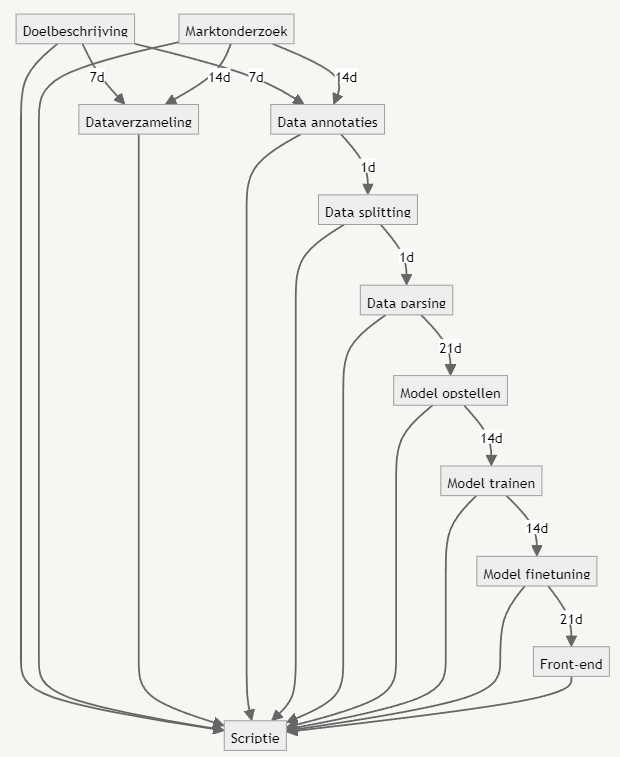
\includegraphics[width=8cm]{flow_new}
\\

\subsection{Gantt-chart}
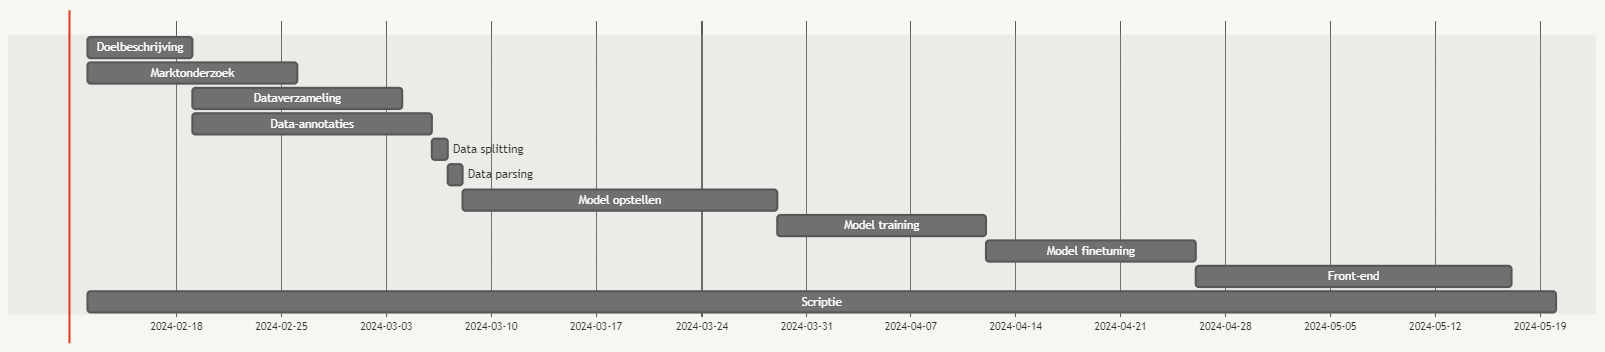
\includegraphics[width=8cm]{gantt_new}
\\\\

%---------- Verwachte resultaten ----------------------------------------------
\section{Verwacht resultaat, conclusie}%
\label{sec:verwachte_resultaten}

% Hier beschrijf je welke resultaten je verwacht. Als je metingen en simulaties uitvoert, kan je hier al mock-ups maken van de grafieken samen met de verwachte conclusies. Benoem zeker al je assen en de onderdelen van de grafiek die je gaat gebruiken. Dit zorgt ervoor dat je concreet weet welk soort data je moet verzamelen en hoe je die moet meten.

% Wat heeft de doelgroep van je onderzoek aan het resultaat? Op welke manier zorgt jouw bachelorproef voor een meerwaarde?

% Hier beschrijf je wat je verwacht uit je onderzoek, met de motivatie waarom. Het is \textbf{niet} erg indien uit je onderzoek andere resultaten en conclusies vloeien dan dat je hier beschrijft: het is dan juist interessant om te onderzoeken waarom jouw hypothesen niet overeenkomen met de resultaten.


% De laatste stap om te bepalen of het afgelegde onderzoek succesvol was, is het ontwikkelen van een front-end die het mogelijk maakt om het model te gebruiken en de resultaten te visualiseren.
% In deze visualisatie zal het mogelijk zijn om de wedstrijd te streamen naar een platform zoals Twitch of YouTube, de score bij te houden, de statistieken van spelers bij te houden en de wedstrijd te analyseren.
% In deze visualisatie zal het mogelijk zijn om de wedstrijd live en achteraf te analyseren. Onder live analyses worden spelers, referees, de bal, $\ldots$ beschouwd, terwijl de statistieken achteraf zullen bestaan uit eindresultaten zoals score per speler, rebounds, het aantal minuten dat een speler op het veld heeft gestaan, aantal vrije worpen, $\ldots$ .


Als laatste stap om het succes van het uitge-\\voerde onderzoek te beoordelen, zal een front-end worden ontwikkeld waarmee het model kan worden toegepast en de resultaten kunnen \\worden gevisualiseerd. 
In deze visuele weergave is het mogelijk om zowel live als achteraf de \\basketbalwedstrijd te analyseren.


Live-analyse omvat het volgen van spelers, \\scheidsrechters, de bal, enz., terwijl achteraf \\gegenereerde statistieken de individuele punten van de spelers, rebounds, speeltijd per speler, \\aantal genomen vrije worpen en meer omvatten. Er zal ook gekeken worden in hoeverre het \\mogelijk is om (als tafelofficial) manueel de scores aan te passen indien er te veel of te weinig punten aan de ploegen zijn toegekend door het systeem.


Voor de analyse achteraf wordt een functiona-\\liteit toegevoegd waarmee coaches en spelers een opname van de wedstrijd kunnen uploaden. Deze opname wordt verwerkt door het model en de resulterende analyse wordt gepresenteerd in de front-end. Dit stelt coaches en spelers in staat om te begrijpen waar eventuele struikelpunten in de wedstrijd lagen en te reflecteren op gemaakte tactische beslissingen. 

De gecollecteerde statistieken en inzichten uit de analyses kunnen bijgevolg dienen als waardevolle input voor het aanpassen van de doordeweekse trainingen en het verbeteren van \\prestaties in toekomstige wedstrijden.


%---------- Vooruitstrevende veranderingen ----------------------------------------------
\section{Baanbrekende innovaties}
\label{sec:vooruitstrevende_veranderingen}
%Wanneer dit project tot een goed einde wordt gebracht, is er nog ruimte voor toekomstige mogelijkheden.
Bij succesvolle afronding van dit project \\openen er nieuwe deuren voor innovaties. Dit zijn een aantal van de mogelijkheden:
\begin{itemize}
    \item \textbf{Game Highlights Creatie:} het model kan worden uitgebreid om automatisch hoogte-\\punten van de wedstrijd te creëren waardoor boeiende momenten snel toegankelijk zijn voor de clubs en hun fans
    \item \textbf{Livestream Opties:} de implementatie van functies voor live streaming naar populaire platforms zoals YouTube, Twitch, Facebook, enz., waardoor fans de wedstrijd realtime en van thuis uit kunnen volgen
    \item \textbf{Referee Handgebaren Analyse:} door handgebaren van scheidsrechters in 'close sight' te monitoren, kan het model lichaamstaal interpreteren om verschillende soorten \\fouten te herkennen en deze aan specifieke spelers te koppelen\\\\\\\\
    \item \textbf{Uitgebreide Spelersactie Analyse:} het \\model kan worden getraind om gedetailleerde acties van spelers bij te houden zoals lopen, stilstaan, dribbelen, verdedigen, enz., om meer diepgaande en persoonlijke \\statistieken te generen
    \item \textbf{Intelligent Area Prediction:} de toepassing van intelligente voorspellingen op de belangrijkste locaties op het speelveld vast te \\leggen via camera's waardoor specifieke \\zones en hotspots kunnen worden ge-\\identificeerd
\end{itemize}
Deze voorgestelde innovaties breiden de functiona-liteiten van het huidige model uit en verbeteren de algehele basketbalervaring voor zowel fans als professionals.\\




